\begin{frame}
    \frametitle{Relaxation Path}
    % a comment
    \begin{figure}[htbp!]
      \begin{center}
        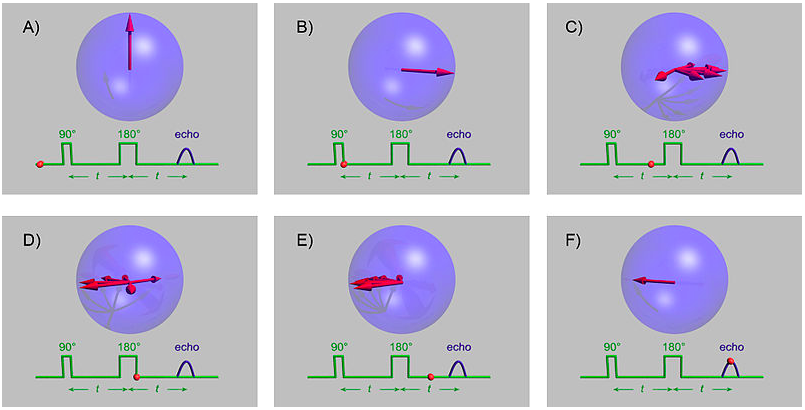
\includegraphics[width=\linewidth]{./images/figures/theory/relax.png}
      \end{center}
            \caption{General Relaxation Path \cite{spin_echo}}
      \label{fig:relax}
    \end{figure}
  \end{frame}

\begin{frame}
    \frametitle{Frequency Deviation}
    % Talk about the wacky result from sample D around 0.17, what's doing 
    \begin{figure}[htbp!]
        \begin{center}
            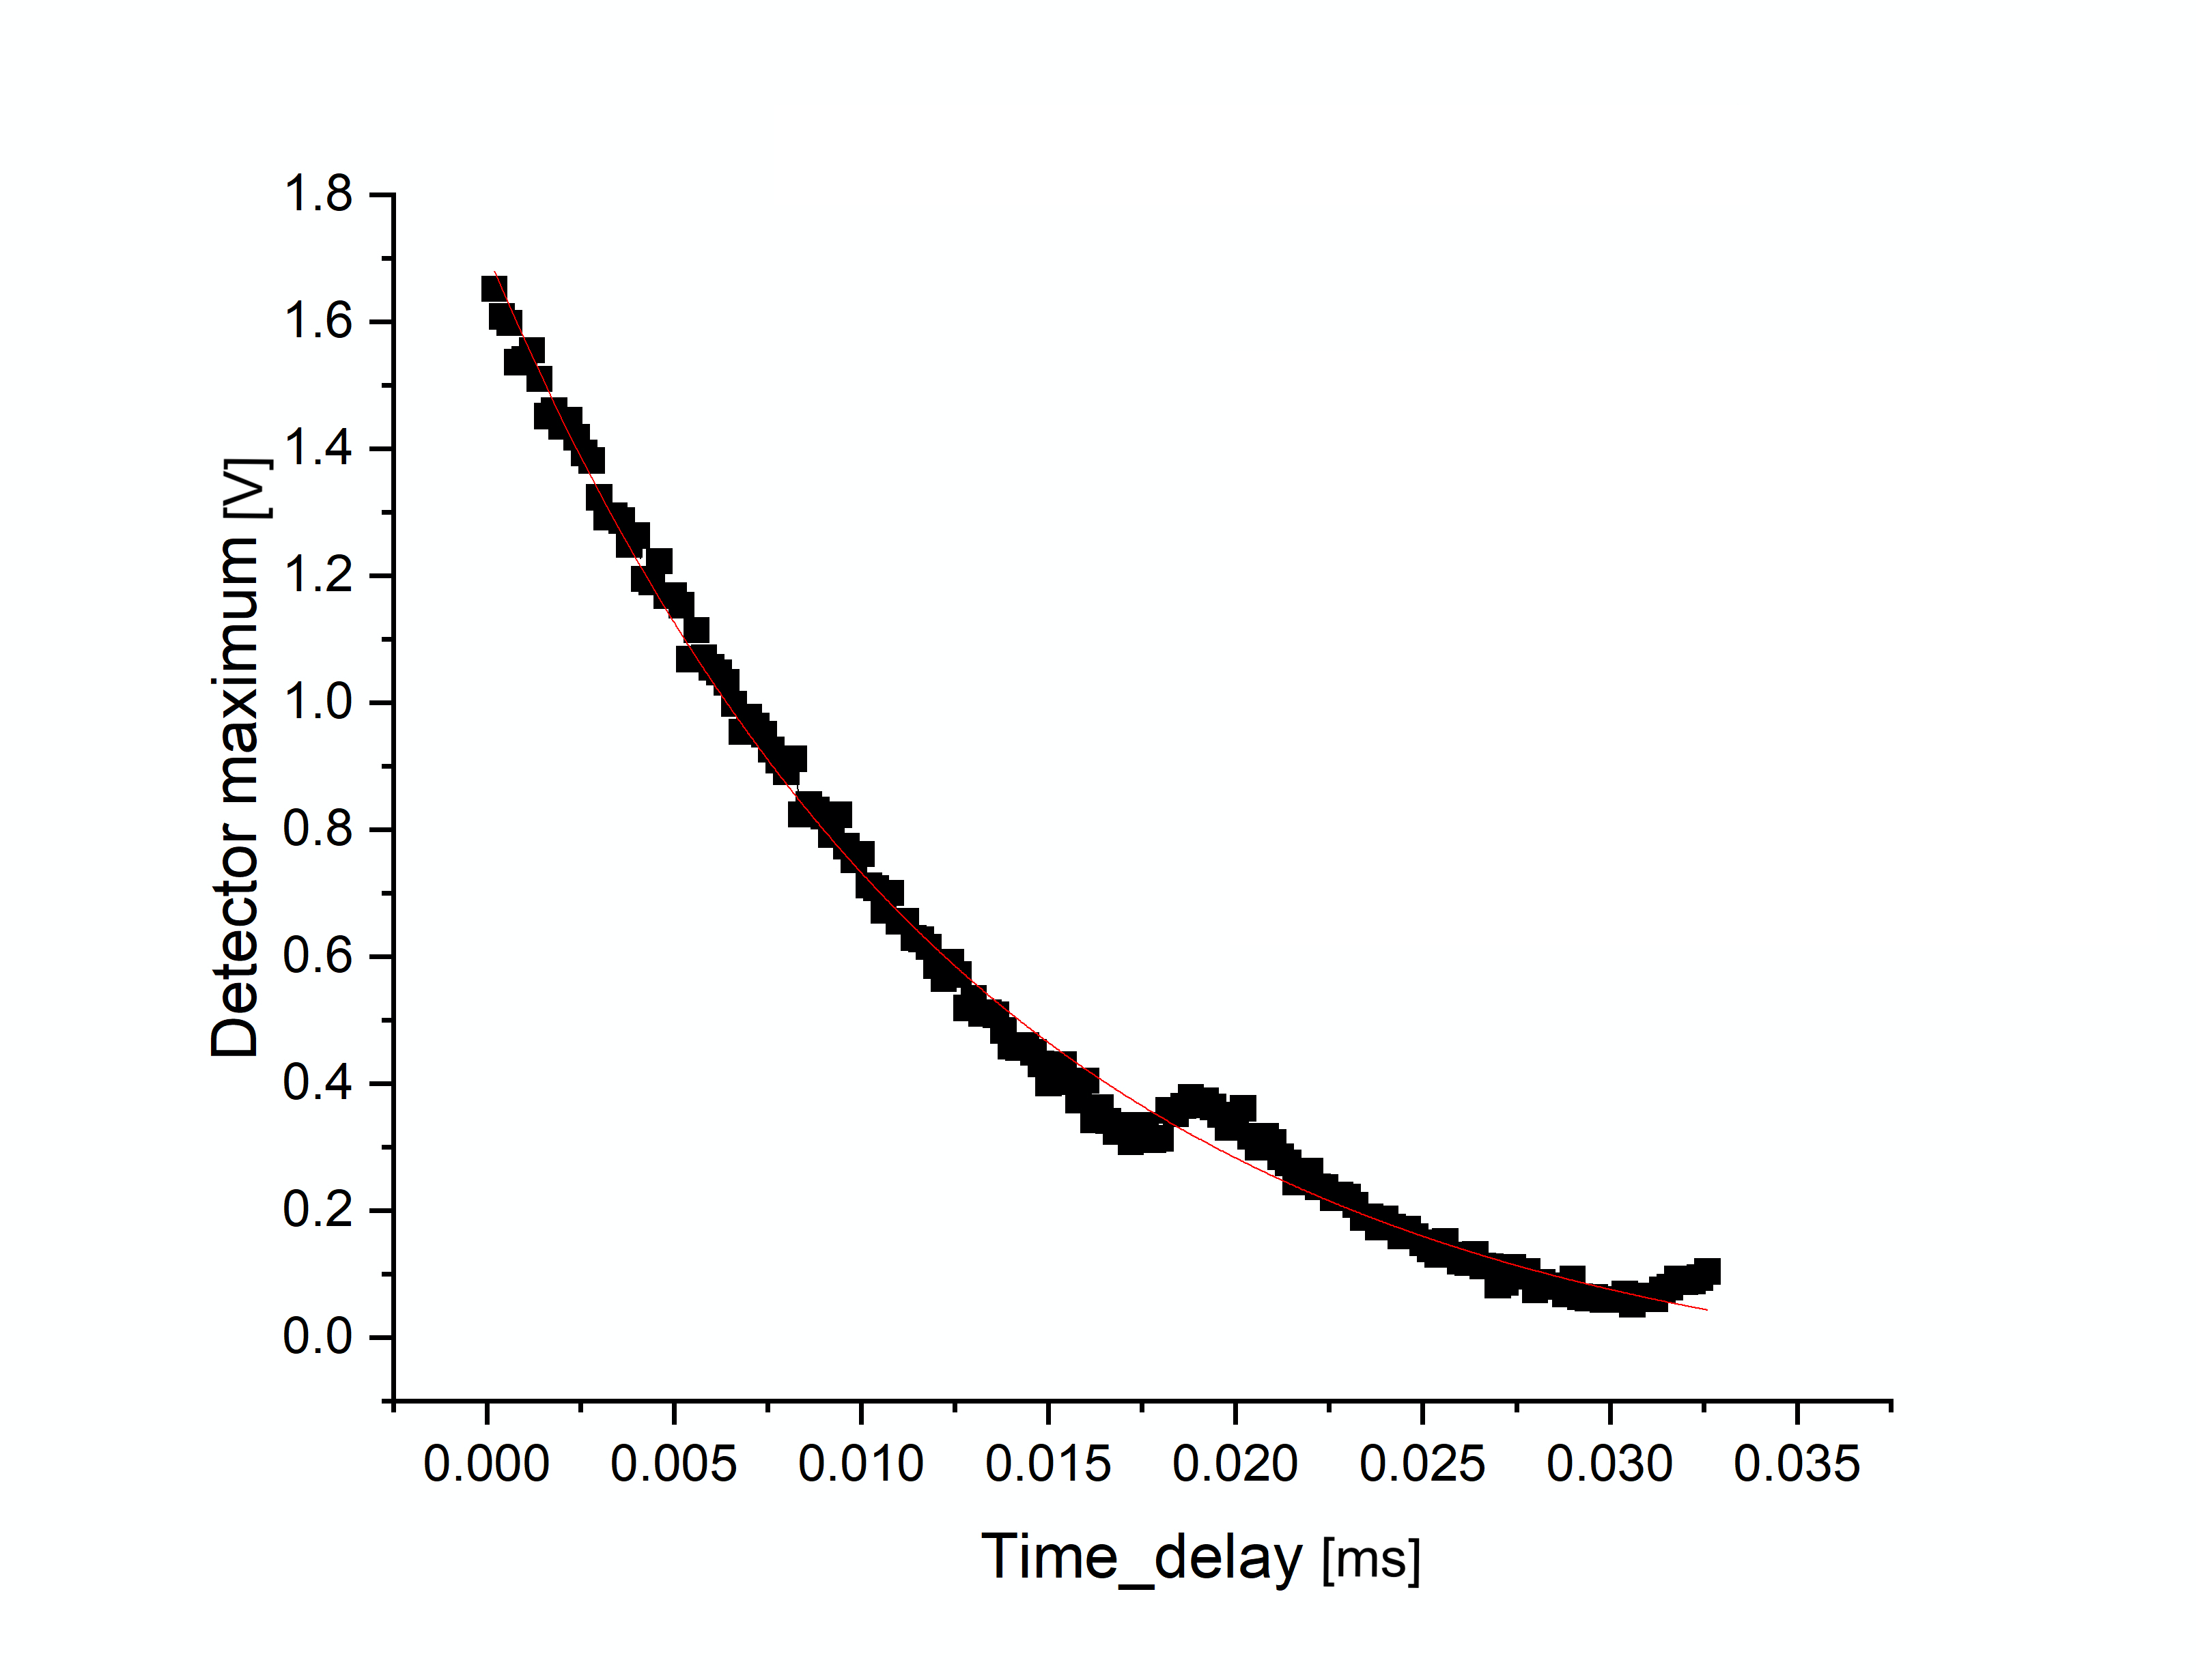
\includegraphics[scale=0.31]{./images/figures/theory/d-t1.png}
        \end{center}
                \caption{Sample D [$ 3.37 \pm 1.6 x 10^{-2}$]:$ T_1$}
        \label{fig:d_t1}
    \end{figure}
\end{frame}

\begin{frame}
    \frametitle{Exceeding Relaxation Time}
    \begin{figure}[htbp!]
        \begin{center}
            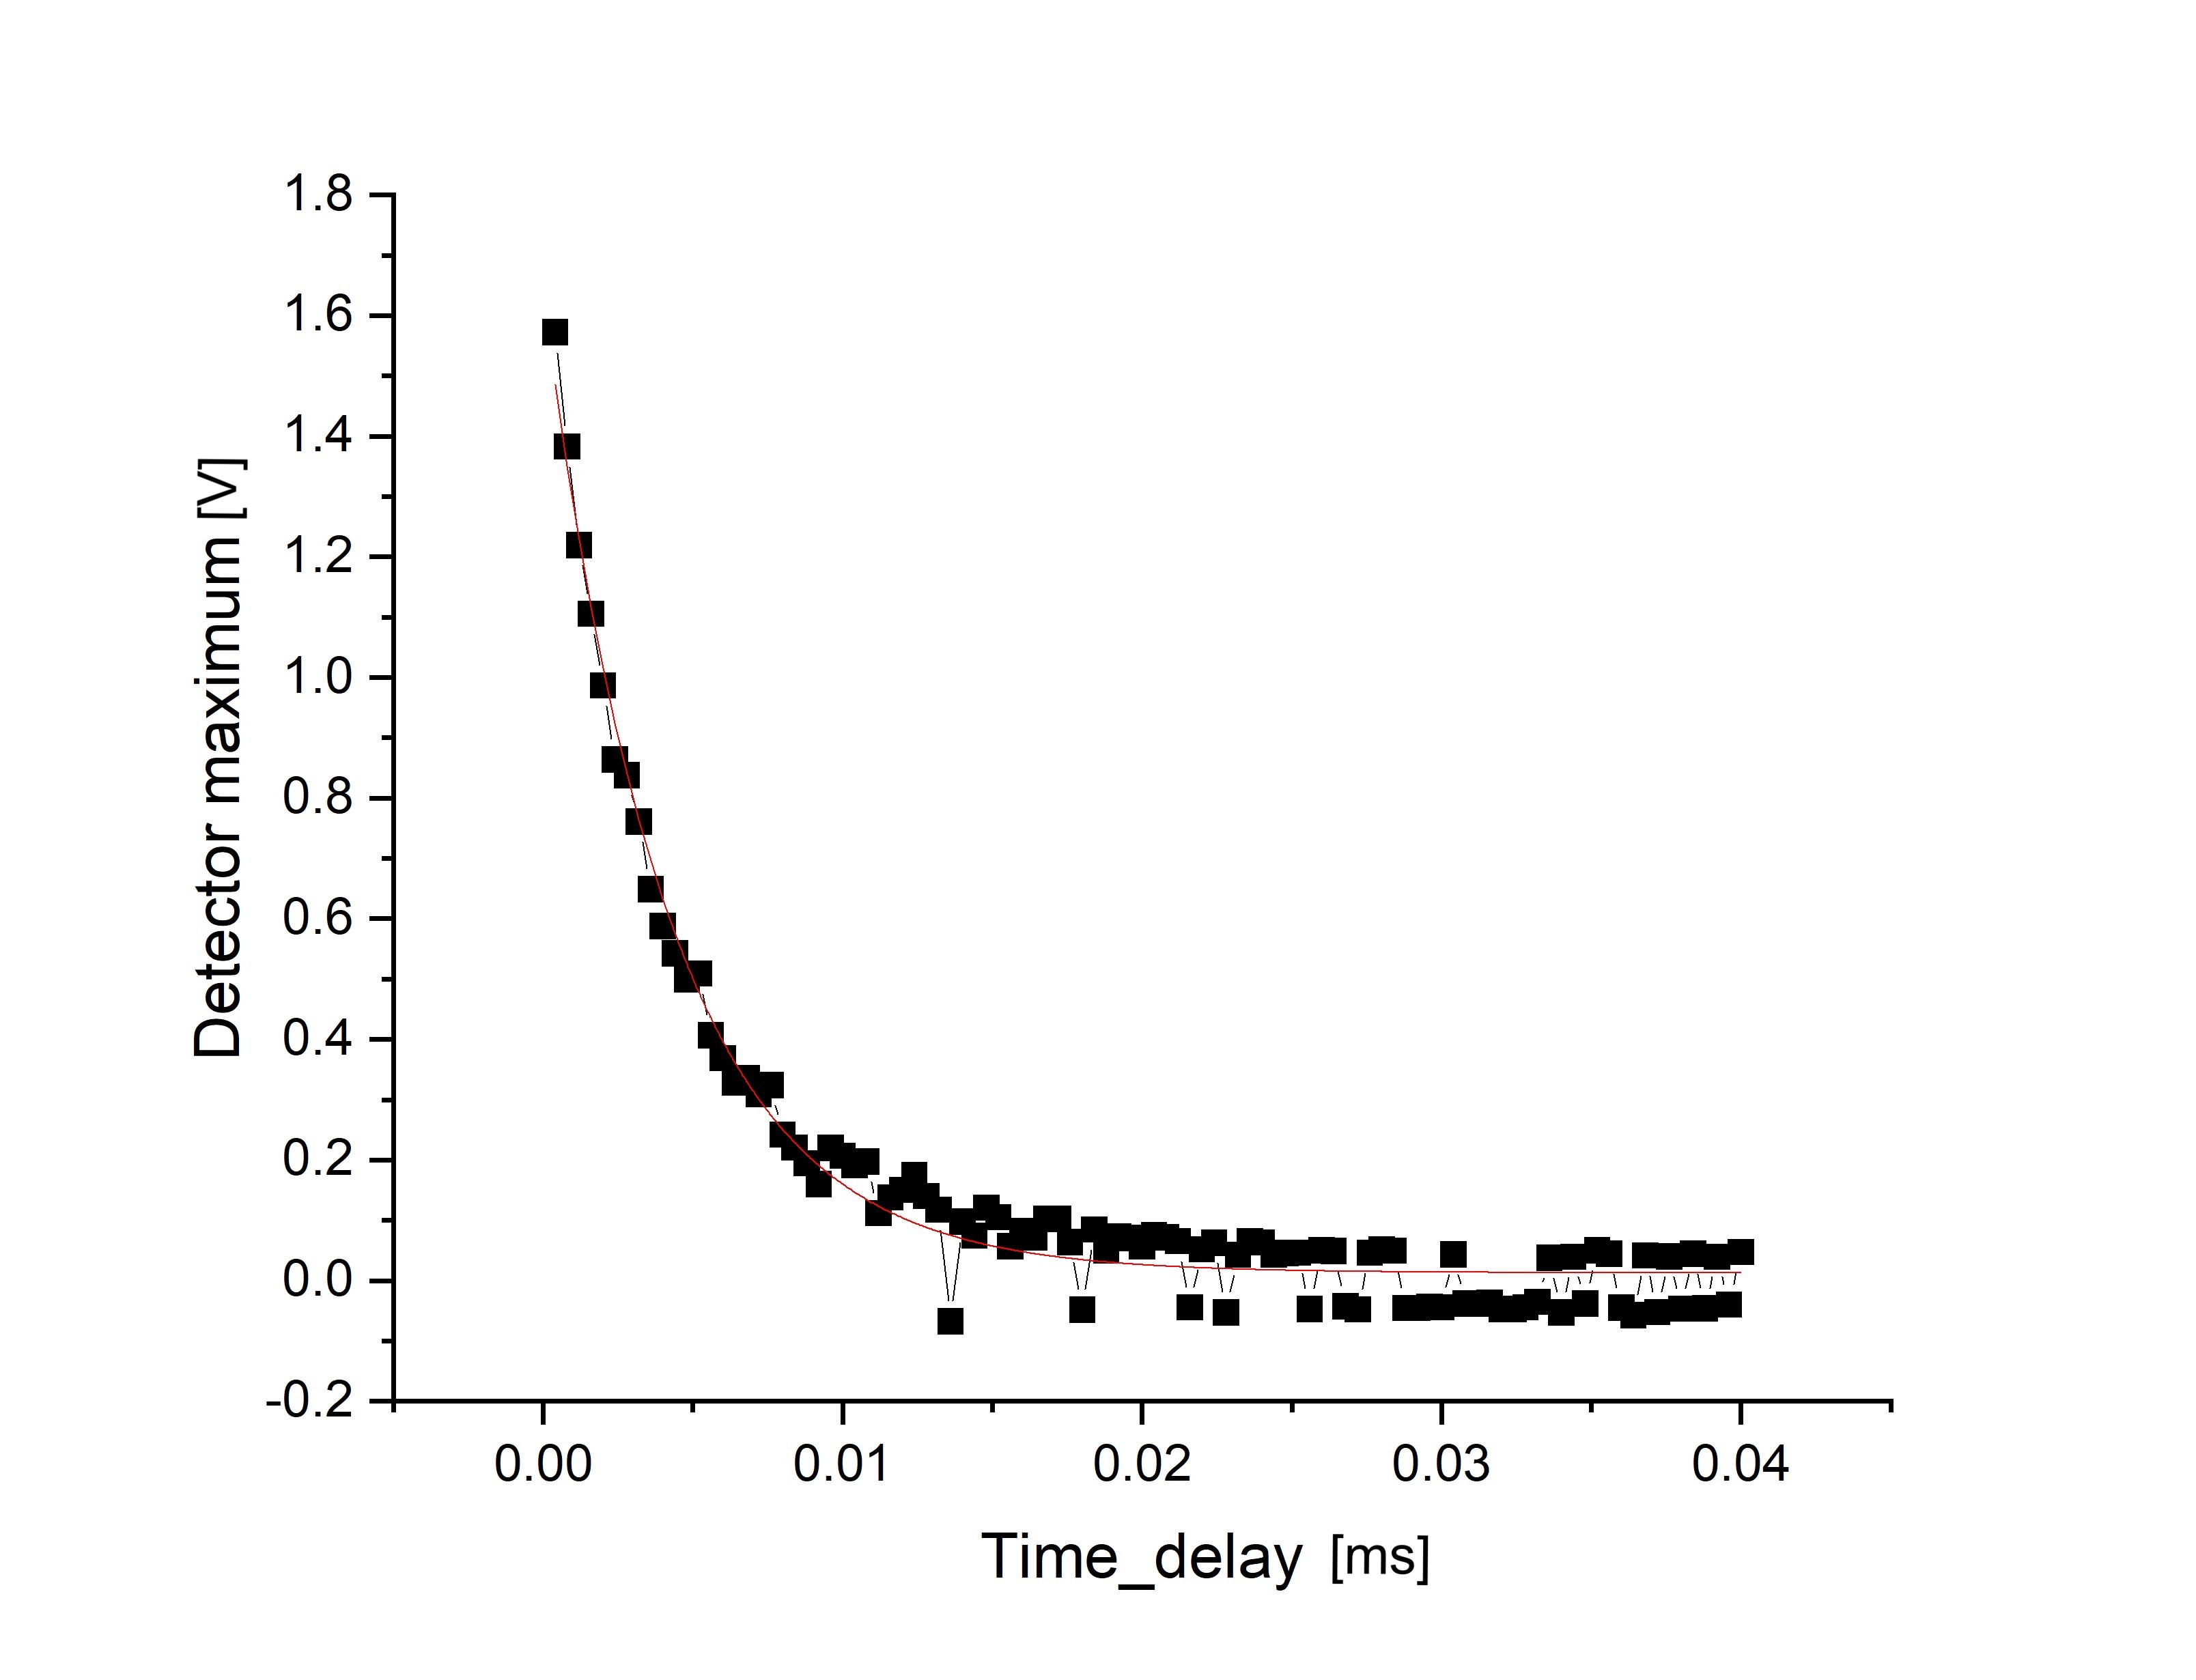
\includegraphics[scale=0.07]{./images/figures/t_plots_appendix/a_t-2.jpg}
        \end{center}
                \caption{Sample A [$ 34.0 \pm 6.0 x 10^{-2}$]:$ T_2$}
        \label{fig:a_t2}
    \end{figure}
\end{frame}